\documentclass{beamer}
\usetheme{metropolis}

\title{Learning Contact Dynamics with LCP Constraint Relaxations}
\author{Samuel Pfrommer, Michael Posa}
\institute{DAIR Lab at the University of Pennsylvania}
\date{\today}

\usepackage{tikz}
\usetikzlibrary{arrows}
\usetikzlibrary{arrows.meta}

\usepackage{caption}

\usepackage{listings}

\begin{document}

\lstset{language=C++,
    basicstyle=\ttfamily,
    keywordstyle=\color{blue}\ttfamily,
    stringstyle=\color{red}\ttfamily,
    commentstyle=\color{black!50!green}\ttfamily,
    morecomment=[l][\color{magenta}]{\#}
}

\begin{frame}
    \titlepage
\end{frame}

\begin{frame}
    \frametitle{Overview}
    \begin{itemize}
        \item Problems with manipulation
        \item Existing approaches
        \item How are we learning?
        \item What are we learning?
    \end{itemize}
\end{frame}

\section{Manipulation overview}

\begin{frame}
    \frametitle{Problems with manipulation}
    \begin{itemize}
        \item Sudden changes in dynamics when making/breaking contact 
        \item Inconsistencies with Coulomb friction (Painlev\'{e} paradox)
        \item Many simultaneous contacts
        \item Stick/slip transitions
    \end{itemize}
\end{frame}

\begin{frame}
    \frametitle{Existing approaches}
    \begin{columns}[t]
        \begin{column}{0.33\textwidth}
            \textbf{Learned}
            \begin{itemize}
                \item Often in context of policy learning
                \item Slow and data innefficient
                \item Doesn't leverage existing understanding of contact dynamics
            \end{itemize}
        \end{column}

        \begin{column}{0.33\textwidth}
            \textbf{Hybrid}
            \begin{itemize}
                \item Best of both worlds
                \item Residual physics
                \item Sim-to-real
                \item \textbf{Differentiation through LCPs}
            \end{itemize}
        \end{column}

        \begin{column}{0.33\textwidth}
            \textbf{Analytical}
            \begin{itemize}
                \item Only an approximation
                \item Doesn't fully capture real-world phenomena
            \end{itemize}
        \end{column}

    \end{columns}
\end{frame}

\begin{frame}
    \frametitle{GridPoint, GridLinePoint, GridFloatPoint}
    \begin{figure}
        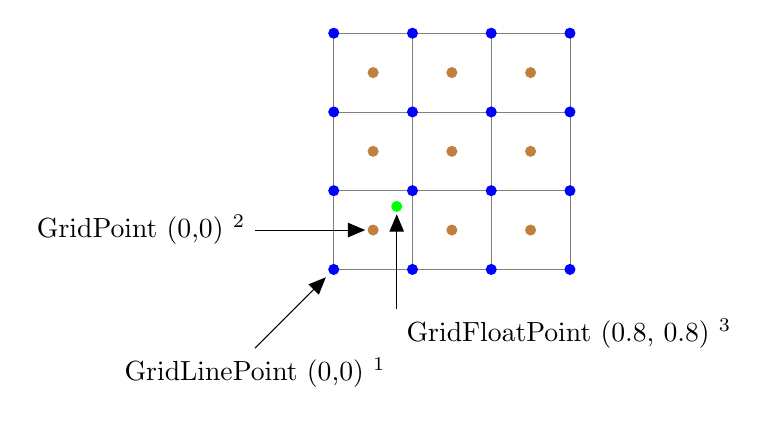
\begin{tikzpicture}
            \draw[gray,very thin] (0,0) grid (3,3);
            \foreach \x in {0,1,...,3}{
                \foreach \y in {0,1,...,3}{
                    \fill[blue] (\x,\y) circle[radius=2pt];
            }}
            \node[anchor=north] at (-1,-1) {GridLinePoint (0,0) \footnotemark};
            \draw[arrows={-triangle 45}] (-1,-1) -- (-0.1,-0.1);
            \foreach \x in {0,1,...,2}{
                \foreach \y in {0,1,...,2}{
                    \fill[brown] (\x+0.5,\y+0.5) circle[radius=2pt];
            }}
            \node[anchor=east] at (-1,0.5) {GridPoint (0,0) \footnotemark};
            \draw[arrows={-triangle 45}] (-1,0.5) -- (0.4,0.5);
            \fill[green] (0.8, 0.8) circle[radius=2pt];
            \node[anchor=north west] at (0.8, -0.5) {GridFloatPoint (0.8, 0.8) \footnotemark};
            \draw[arrows={-triangle 45}] (0.8,-0.5) -- (0.8,0.7);
        \end{tikzpicture}
    \end{figure}

    \footnotetext[1]{A new type}
    \footnotetext[2]{Reuse of existing occupancy-grid GridPoint}
    \footnotetext[3]{Reuse of existing occupancy-grid grid\_coord\_t}
\end{frame}

\begin{frame}
    \frametitle{Derived geometries}
    \begin{itemize}
        \item All associated geometries have names derived from point type and characteristics
            \begin{itemize}
                \item GridPointSegment vs GridLineSegment
                \item GridPointRing/GridPointRing90 vs GridLineRing/GridLineRing90
                \item GridPointPoly/GridPointPoly90 vs GridLinePoly/GridLinePoly90
                \item etc...
            \end{itemize}
    \end{itemize}
\end{frame}

\begin{frame}
    \frametitle{Gridline geometries examples}
    \begin{figure}
        \resizebox{1\textwidth}{0.75\textwidth}{
            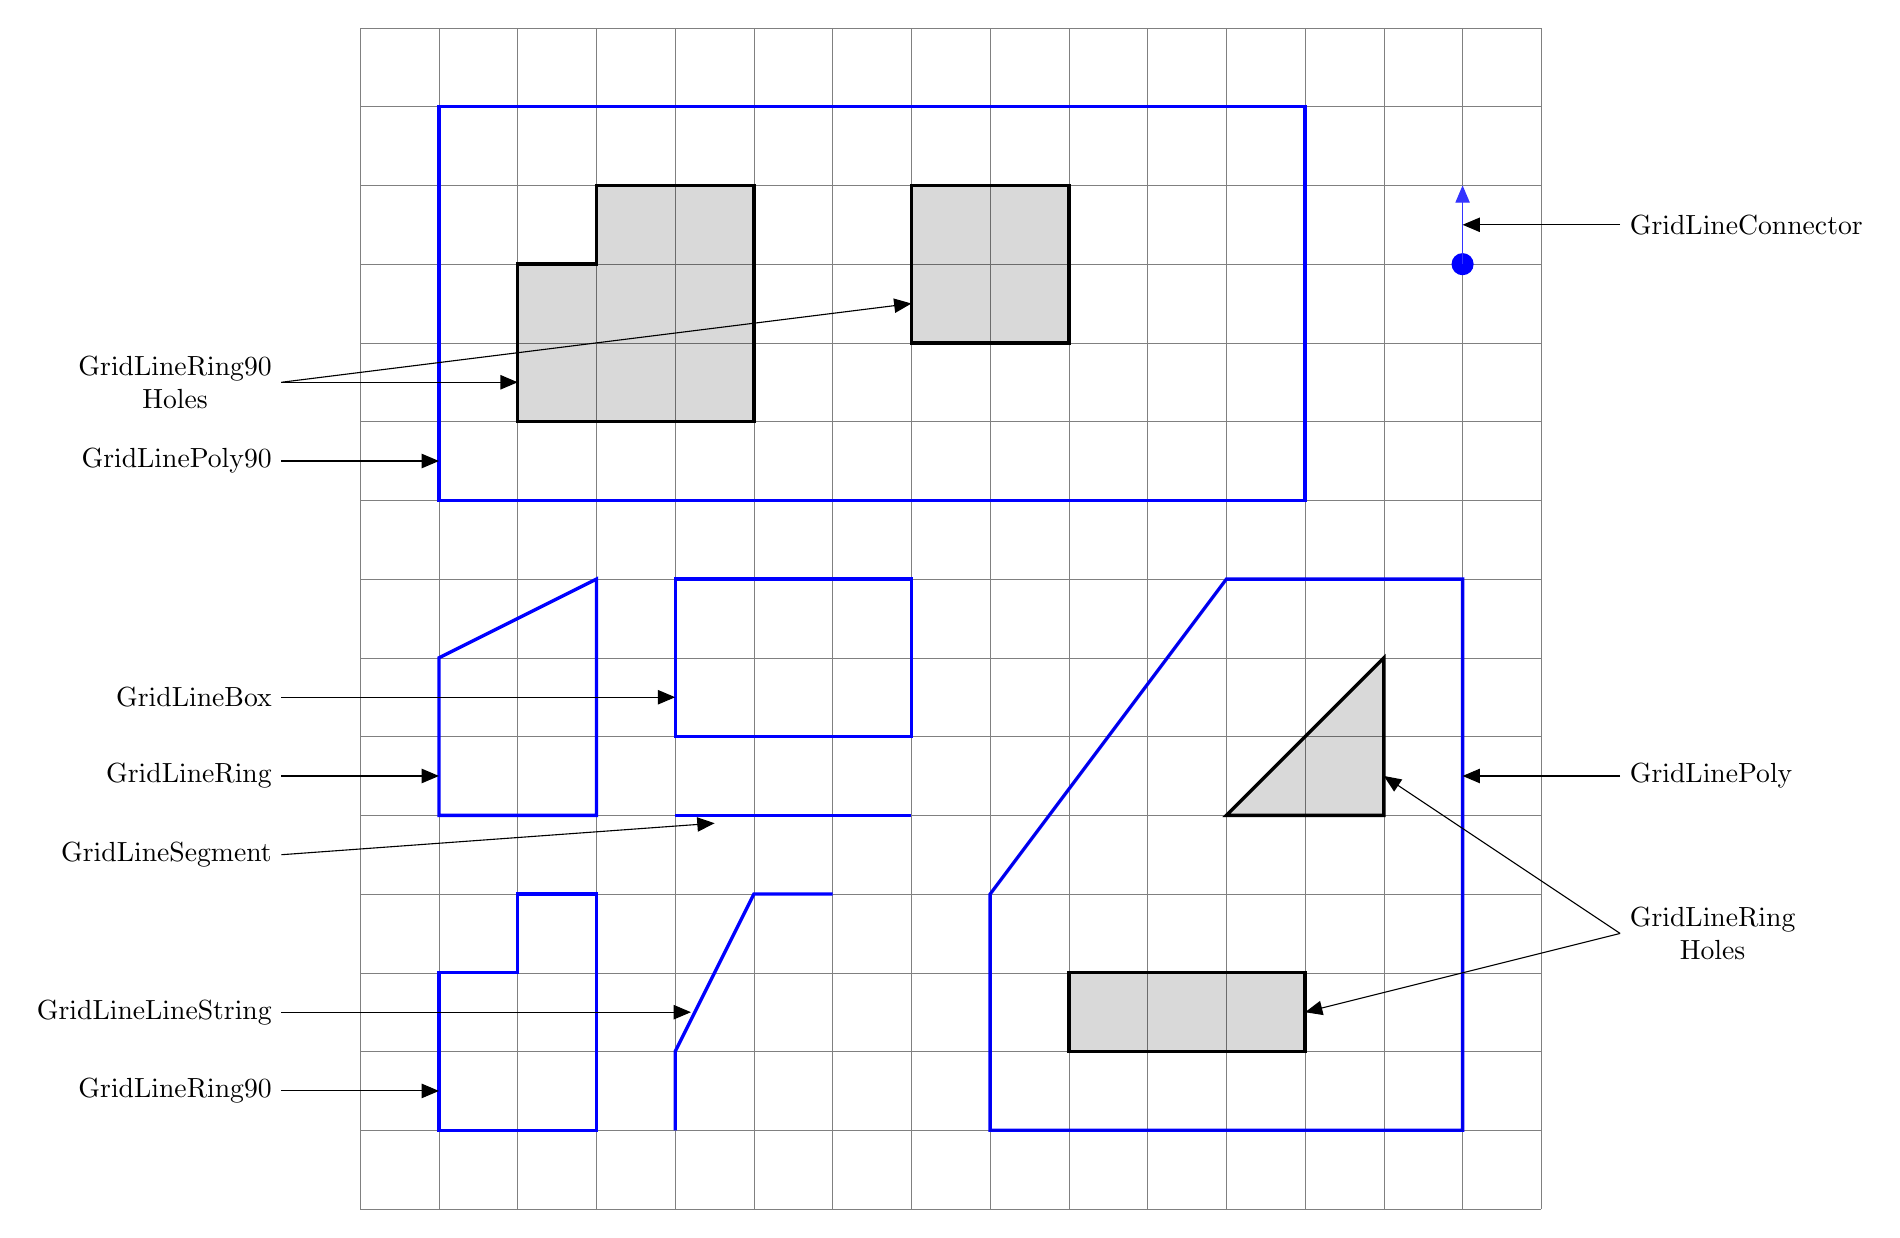
\begin{tikzpicture}
                \draw[gray, very thin] (0,0) grid (15,15);

                \draw[blue, very thick] (1,1) -- (1,3) -- (2,3) -- (2,4) -- (3,4) -- (3,1) -- cycle;
                \node[anchor=east] at (-1,1.5) {GridLineRing90};
                \draw[arrows={-triangle 45}] (-1,1.5) -- (1,1.5);

                \draw[blue, very thick] (1,5) -- (1,7) -- (3,8) -- (3,5) -- cycle;
                \node[anchor=east] at (-1,5.5) {GridLineRing};
                \draw[arrows={-triangle 45}] (-1,5.5) -- (1,5.5);

                \draw[blue, very thick] (1,9) -- (1,14) -- (12,14) -- (12,9) -- cycle;
                \node[anchor=east] at (-1,9.5) {GridLinePoly90};
                \draw[arrows={-triangle 45}] (-1,9.5) -- (1,9.5);
                \draw[black, very thick] (2,10) -- (2,12) -- (3,12) -- (3,13) -- (5,13) -- (5,10) -- cycle;
                \filldraw[black, opacity=0.15] (2,10) -- (2,12) -- (3,12) -- (3,13) -- (5,13) -- (5,10) -- cycle;
                \draw[black, very thick] (7,11) rectangle (9,13);
                \fill[black, opacity=0.15] (7,11) rectangle (9,13);

                \node[anchor=east, align=center] at (-1,10.5) {GridLineRing90\\Holes};
                \draw[arrows={-triangle 45}] (-1,10.5) -- (2,10.5);
                \draw[arrows={-triangle 45}] (-1,10.5) -- (7,11.5);

                \draw[blue, very thick] (4,6) rectangle (7,8);
                \node[anchor=east] at (-1,6.5) {GridLineBox};
                \draw[arrows={-triangle 45}] (-1,6.5) -- (4,6.5);

                \draw[blue, very thick] (4,1) -- (4,2) -- (5,4) -- (6,4);
                \node[anchor=east] at (-1,2.5) {GridLineLineString};
                \draw[arrows={-triangle 45}] (-1,2.5) -- (4.2,2.5);

                \draw[blue, very thick] (4,5) -- (7,5);
                \node[anchor=east] at (-1,4.5) {GridLineSegment};
                \draw[arrows={-triangle 45}] (-1,4.5) -- (4.5,4.9);

                \fill[blue] (14,12) circle[radius=4pt];
                \draw[blue!80, arrows={-triangle 45}] (14,12) -- (14,13);
                \node[anchor=west] at (16,12.5) {GridLineConnector};
                \draw[arrows={-triangle 45}] (16,12.5) -- (14,12.5);


                \draw[blue, very thick] (8,1) -- (8,4) -- (11, 8) -- (14,8) -- (14,1) -- cycle;
                \node[anchor=west] at (16,5.5) {GridLinePoly};
                \draw[arrows={-triangle 45}] (16,5.5) -- (14,5.5);
                \draw[black, opacity=0.15] (8,1) -- (8,4) -- (11, 8) -- (14,8) -- (14,1) -- cycle;
                \draw[black, very thick] (9,2) rectangle (12,3);
                \fill[black, opacity=0.15] (9,2) rectangle (12,3);
                \draw[black, very thick] (11,5) -- (13,7) -- (13,5) -- cycle;
                \filldraw[black, opacity=0.15] (11,5) -- (13,7) -- (13,5) -- cycle;
                \node[anchor=west, align=center] at (16,3.5) {GridLineRing\\Holes};
                \draw[arrows={-triangle 45}] (16,3.5) -- (12,2.5);
                \draw[arrows={-triangle 45}] (16,3.5) -- (13,5.5);
            \end{tikzpicture}
        }
    \end{figure}
\end{frame}

\begin{frame}
    \frametitle{GridPoint and GridLinePoint}
    What is difference between calling boost::geometry::within on a GridPoint and GridLineRing and calling boost::geometry::within on a GridLinePoint and GridLineRing?
    \begin{itemize}
        \item The GridPoint (0,0) is spatially shifted by 0.5f in x and y from the GridLinePoint (0,0)
        \item Before using boost geometry functions relating GridPoints and GridLinePoints, GridPoints must be brought into the GridLinePoint reference frame (see type\_conversions.h)
        \item room-segmentation/geometry/algorithms/within and room-segmentation/geometry/algorithms/covered\_by handle this automatically
    \end{itemize}
\end{frame}

\begin{frame}
    \frametitle{Custom base geometry types}
    \begin{itemize}
        \item Polygon
            \begin{itemize}
                \item Has outer ring and vector of inner rings
                \item Had to be custom since boost geometry polygon hard coded ring types internally (and we really only want a GridLinePoly90 to take GridLineRing90s)
            \end{itemize}
        \item Ring and Linestring
            \begin{itemize}
                \item Implemented using shared\_ptr to point vector rather than inheriting from vector
                \item Allows for shallow copies and conversion between Ring and LineString representation without deep copying points (explain why necessary later)
            \end{itemize}
    \end{itemize}
\end{frame}

\begin{frame}[fragile]
    \frametitle{Sample API}

    \textbf{moment.h}
    \begin{lstlisting}[language=C++, basicstyle=\tiny]
float moment_x(const GridLineRing& ring);
float moment_x(const GridLineRing90& ring);    
    \end{lstlisting}

    \textbf{moment.cpp}
    \begin{lstlisting}[language=C++, basicstyle=\tiny]
template <typename RingT> float moment_x_generic(const RingT& ring)
{
    float sum = 0.0f;
    for (size_t i = 0; i < ring.size() - 1; i++)
    {
        float x_i, y_i, x_in, y_in = ...
        sum += (y_i*y_i + y_i*y_in + y_in*y_in) * (x_i*y_in - x_in*y_i);
    }
    sum = sum / 12.0f;
    return -sum;
}
float moment_x(const GridLineRing& ring) 
{
    return moment_x_generic(ring);
}
float moment_x(const GridLineRing90& ring)
{
    return moment_x_generic(ring);
}
    \end{lstlisting}
\end{frame}

\begin{frame}[fragile]
    \frametitle{Shallow copy usage scenarios}
    \begin{itemize}
        \footnotesize
    \item Do \textbf{not} need type reinterpreting for generic APIs operating on geometries
    \item Might need type reinterpreting to set an existing geometry variable
    \item Use sparingly: really should only convert rectilinear to nonrectilinear
\end{itemize}
\textbf{regionWshed.h}
\begin{lstlisting}[language=C++, basicstyle=\tiny]
class RegionWshed
{
    void set_simplified_boundary(const GridLinePoly& p);
    void set_simplified_boundary(const GridLinePoly90& p);

    GridLinePoly _simplified_boundary;
}
\end{lstlisting}
\textbf{regionWshed.cpp}
\begin{lstlisting}[language=C++, basicstyle=\tiny]
void RegionWshed::set_simplified_boundary(const navgeometry::GridLinePoly90& p)
{
    _simplified_boundary = reinterpret_poly<GridLinePoly>(p);
}
void RegionWshed::set_simplified_boundary(const navgeometry::GridLinePoly& p)
{
    _simplified_boundary = p;
}
\end{lstlisting}
\end{frame}

\begin{frame}[fragile]
    \frametitle{Reinterpreting geometries}
    \begin{itemize}
        \item LineString and Ring are both just vectors of points
        \item Boost geometry algorithms sometimes behave differently and one behavior might be preferred
        \item Use helper function reinterpret\_geometry
    \end{itemize}
    \begin{lstlisting}[language=C++, basicstyle=\tiny]
GridLineRing90 ring({{0, 0}, {0, 4}, {4, 4}, {4, 0}, {0, 0}});
GridLineLineString ring_reinterpreted = reinterpret_ring<GridLineLineString>(ring);
// Outputs zero since point is inside ring
cout << boost::geometry::distance(GridLinePoint(1, 1), ring1) << endl;
// Outputs one (desired)
cout << boost::geometry::distance(GridLinePoint(1, 1), ring1_reinterpreted) << endl;
    \end{lstlisting}
\end{frame}

\section{API structure}

\begin{frame}[fragile]
    \frametitle{Interacting with grids}
    \textbf{Traversal directions}
    \begin{lstlisting}[language=C++, basicstyle=\tiny]
enum class GridDir { RIGHT = 0, UP = 1, LEFT = 2, DOWN = 3 };
enum class DiagDir { UPRIGHT = 0, UPLEFT = 1, DOWNLEFT = 2, DOWNRIGHT = 3 };
enum class TurnDir { STRAIGHT = 0, LEFT = 1, REVERSE = 2, RIGHT = 3 };
    \end{lstlisting}
    \textbf{grid\_traversal.h}
    \begin{itemize}
        \item Various utility functions for traversing grids
    \end{itemize}
    \textbf{type\_conversions.h}
    \begin{itemize}
        \item Converting GridPoints to GridFloatPoints
        \item Also for shallow converting different types of geometries
    \end{itemize}
\end{frame}

\begin{frame}
    \frametitle{Boost geometry wrappers}
    \begin{itemize}
        \item Calling boost::geometry::within(GridPoint p, GridLineRing r) is \textbf{WRONG}
        \item Say the GridPoint is (2,0), and a segment of the GridLineRing goes from (0,0) to (4,0)
        \item Boost geometry will say that the point is not within the polygon since it's on the boundary, even though the GridPoint should be shifted up and to the right by 0.5 and hence be within
        \item Same applies to boost::geometry::covered\_by and other similar functions
        \item Solution: use custom navgeometry::within or navgeometry::covered\_by (in geometry/algorithms)
    \end{itemize}
\end{frame}

\begin{frame}
    \frametitle{Adding algorithms}
    \small
    \begin{itemize}
        \item All algorithms go in geometry/algorithms
        \item Try to use verbs for the file names wherever possible
        \item \textbf{ONE} algorithm, \textbf{ONE} .h/.cpp file pair
        \item .h file declares what geometry types the algorithm can take
        \item If implementations for rectilinear/nonrectilinear geometries are different, have two separate implementations in .cpp file; otherwise, have a templatized version \textbf{IN THE CPP FILE} and call it from the two specific functions (see sample API)
        \item If you really want a boost geometry type function which will take anything and try to run an algorithm on it (\textbf{NOT RECOMMENDED}), make it templatized in the header
        \item As of writing within/covered\_by and a few other algorithms don't define functions taking GridPointRing and GridPointPoly since it's not needed at the moment, even though it could (and probably should) be added
    \end{itemize}
\end{frame}

\begin{frame}[fragile]
    \frametitle{Utilities for writing generalized algorithms}
    \begin{itemize}
        \item Get\_x and get\_y for points (legacy point objects have different ways of accessing x and y)
        \item Typedef for child geometries (e.g., ring\_type in Polygon)
            \begin{itemize}
                \item Useful if you want to add a ring to a generalized Polygon or something along those lines
            \end{itemize}
    \end{itemize}
    \begin{lstlisting}[language=C++, basicstyle=\tiny]
template <typename Poly>
void frankenstein(Poly* poly)
{
    typename Poly::point_type point(get_x((*poly).outer()[0]) + 5,
                                    get_y((*poly).outer()[0]));
    cout << boost::geometry::dsv(point) << endl;
    typename Poly::ring_type ring;
    boost::geometry::read_wkt("POLYGON((0 0, 0 4, 2 0))", ring);
    poly->inners().push_back(std::move(ring));
}
...
GridLinePoly90 poly({GridLineRing90({{0,0}})});
frankenstein(&poly);
    \end{lstlisting}
\end{frame}

\section{Boundary extraction}

\begin{frame}
    \frametitle{Requirements}
    \begin{itemize}
        \item Should take DImage and find GridLineRings surrounding regions of GridPoints with the same label (called a \textbf{boundary})
        \item The GridLineLineString sandwiched between two different-labeled regions should be returned as a \textbf{border} except when one side is a region of zeroes (obstacle)
        \item Regions within regions should become holes in the parent region's polygon (but also be returned as region boundaries)
        \item Obstacles should become holes, but not be returned as region boundaries or have borders
    \end{itemize}
\end{frame}

\begin{frame}
    \frametitle{Extracting a boundary}
    \begin{itemize}
        \item Start at lower-left hand GridLinePoint
        \item Start moving with GridDir::UP
        \item Want to trace out boundary clockwise
        \item Regions connected diagonally should be parsed as separate regions
    \end{itemize}
    \begin{figure}
        \resizebox{0.8\textwidth}{0.4\textwidth}{
            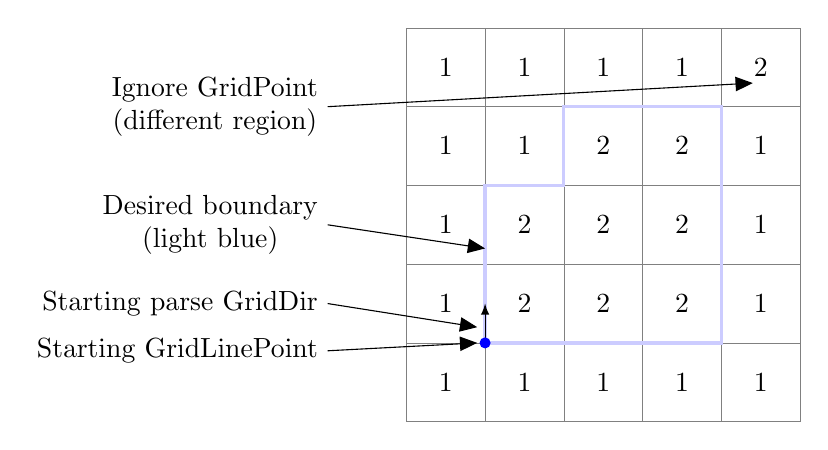
\begin{tikzpicture}
                \draw[gray,very thin] (0,0) grid (5,5);
                \foreach \x in {1,...,3}{
                    \foreach \y in {1,...,2}{
                        \node at (\x+0.5,\y+0.5) {2};
                }}
                \foreach \x in {2,...,3}{
                    \foreach \y in {3}{
                        \node at (\x+0.5,\y+0.5) {2};
                }}
                \foreach \x in {0}{
                    \foreach \y in {0,...,2}{
                        \node at (\x+0.5,\y+0.5) {1};
                }}
                \foreach \x in {0,1}{
                    \foreach \y in {3}{
                        \node at (\x+0.5,\y+0.5) {1};
                }}
                \foreach \x in {0,...,3}{
                    \foreach \y in {4}{
                        \node at (\x+0.5,\y+0.5) {1};
                }}
                \node at (4.5,4.5) {2};
                \foreach \x in {4}{
                    \foreach \y in {0,...,3}{
                        \node at (\x+0.5,\y+0.5) {1};
                }}
                \foreach \x in {1,...,3}{
                    \foreach \y in {0}{
                        \node at (\x+0.5,\y+0.5) {1};
                }}

                \draw[blue!20,very thick] (1,1) -- (1,3) -- (2,3) -- (2,4) -- (4,4) -- (4,1) -- cycle;

                \draw[arrows={-latex}] (1,1) -- (1,1.5);

                \fill[blue] (1,1) circle[radius=2pt];

                \node[anchor=east] at (-1,0.9) {Starting GridLinePoint};
                \draw[arrows={-triangle 45}] (-1,0.9) -- (0.9,1);

                \node[anchor=east] at (-1,1.5) {Starting parse GridDir};
                \draw[arrows={-triangle 45}] (-1,1.5) -- (0.9,1.2);

                \node[anchor=east,align=center] at (-1,2.5) {Desired boundary\\(light blue)};
                \draw[arrows={-triangle 45}] (-1,2.5) -- (1,2.2);

                \node[anchor=east,align=center] at (-1,4) {Ignore GridPoint\\(different region)};
                \draw[arrows={-triangle 45}] (-1,4) -- (4.4,4.3);
            \end{tikzpicture}
        }
    \end{figure}
\end{frame}

\begin{frame}
    \frametitle{Tracing the boundary}
    \begin{itemize}
        \item Consider turning right
            \begin{itemize}
                \item Check whether GridPoint to left of turn belongs to region
                \item If not, make a right turn
                \item If yes, continue to considering going straight
            \end{itemize}
        \item Then consider going straight, then finally make a left turn if necessary
        \item Push back GridLinePoint to boundary whenever make a turn
    \end{itemize}
    \centering
    \begin{figure}
        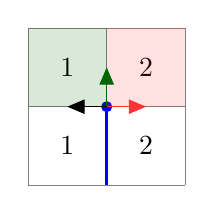
\begin{tikzpicture}
            \draw[gray,very thin] (0,0) grid (2,2);
            \draw[blue,very thick] (1,0) -- (1,1);
            \node at (0.5, 0.5) {1};
            \node at (1.5, 0.5) {2};
            \node at (1.5, 1.5) {2};
            \node at (0.5, 1.5) {1};
            \fill[blue] (1,1) circle[radius=2pt];


            \draw[red!80,arrows={-triangle 45}] (1,1) -- (1.5,1);
            \fill[red!80,opacity=0.15] (1,1) rectangle (2,2);

            \draw[black!60!green,arrows={-triangle 45}] (1,1) -- (1,1.5);
            \fill[black!60!green,opacity=0.15] (1,1) rectangle (0,2);

            \draw[black,arrows={-triangle 45}] (1,1) -- (0.5,1);
        \end{tikzpicture}
        \centering
        \captionsetup{singlelinecheck=false,justification=centering}
        \caption*{Should pick the green arrow \\ since that's the first direction \\ without a 2 on the lefthand side}
    \end{figure}
\end{frame}

\begin{frame}
    \frametitle{Keeping track of visited gridline connections}
    \begin{itemize}
        \item After every traversal step:
            \begin{itemize}
                \item Mark the GridLineConnector spanning two adjacent GridLinePoints as visited
                \item Also mark the direction in which it was traversed
                \item Each GridLineConnector can be visited up to twice (once from each side)
            \end{itemize}
    \end{itemize}
\end{frame}

\begin{frame}
    \frametitle{Extracting borders}
    \begin{itemize}
        \item Can be done simultaneously with boundary traversal
        \item If the interior point is a zero (obstacle) or the GridLineConnector has been visited, don't extract border
        \item Otherwise, when the label on the outside changes, cap off the current border and start a new one
        \item When hit an obstacle or edge of image, cap off border but don't start new one
        \item Append to current border when turning
    \end{itemize}
\end{frame}
\begin{frame}
    \frametitle{Example border parse result}
    \begin{figure}
        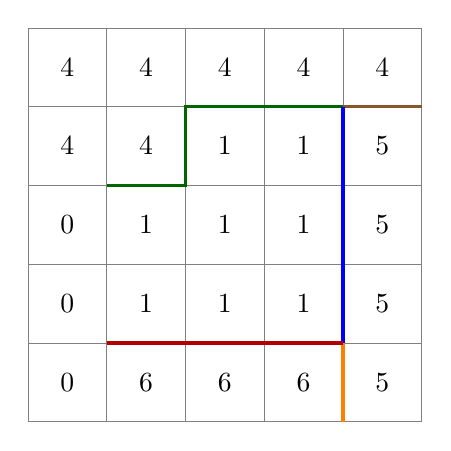
\begin{tikzpicture}
            \draw[gray,very thin] (0,0) grid (5,5);
            \foreach \x in {1,...,3}{
                \foreach \y in {1,...,2}{
                    \node at (\x+0.5,\y+0.5) {1};
            }}
            \foreach \x in {2,...,3}{
                \foreach \y in {3}{
                    \node at (\x+0.5,\y+0.5) {1};
            }}
            \foreach \x in {0}{
                \foreach \y in {0,...,2}{
                    \node at (\x+0.5,\y+0.5) {0};
            }}
            \foreach \x in {0,1}{
                \foreach \y in {3}{
                    \node at (\x+0.5,\y+0.5) {4};
            }}
            \foreach \x in {0,...,4}{
                \foreach \y in {4}{
                    \node at (\x+0.5,\y+0.5) {4};
            }}
            \foreach \x in {4}{
                \foreach \y in {0,...,3}{
                    \node at (\x+0.5,\y+0.5) {5};
            }}
            \foreach \x in {1,...,3}{
                \foreach \y in {0}{
                    \node at (\x+0.5,\y+0.5) {6};
            }}

            \draw[black!60!green, very thick] (1,3) -- (2,3) -- (2,4) -- (4,4);
            \draw[black!30!brown, very thick] (4,4) -- (5,4);
            \draw[orange, very thick] (4,1) -- (4,0);
            \draw[blue, very thick] (4,4) -- (4,1);
            \draw[black!30!red, very thick] (4,1) -- (1,1);
        \end{tikzpicture}
    \end{figure}
\end{frame}

\begin{frame}
    \frametitle{Maintaining the boundary stack}
    \begin{itemize}
        \item How do we know which regions are within other regions (should be holes)?
            \begin{itemize}
                \item Sweep across DImage from left to right, row by row, maintaining a stack of regions
                \item The sweep considers vertical GridLine\textbf{Connectors}, not GridPoints or GridLinePoints
                \item Decide whether to pop, push, or create by checking the traversal direction and whether the right gridpoint's label is on the stack
                \item If a new region is created and a previous region is on the stack, make the new region a hole in the previous one
            \end{itemize}
    \end{itemize}
\end{frame}

\begin{frame}[plain,c]
    \begin{center}
        \Huge Thank you! 
    \end{center}
\end{frame}

\end{document}
